\chapter{Cơ sở lý thuyết}
\label{chap:co_so_ly_thuyet}

Chương này điểm lại các hướng nghiên cứu gần với đề tài (Mục~\ref{sec:nghien-cuu-lien-quan}), rồi trình bày các khái niệm nền tảng (Mục~\ref{sec:khai-niem-nen-tang}) mà Chương~\ref{chap:thiet_ke} đến Chương~\ref{chap:danh_gia} sử dụng. Đó là biểu diễn chung ảnh và văn bản, hàm mất mát tương phản, BM25, tìm kiếm vector gần đúng, tinh chỉnh hiệu quả tham số và các chỉ số đánh giá.

\section{Các nghiên cứu liên quan}
\label{sec:nghien-cuu-lien-quan}

\textbf{Học biểu diễn ảnh và văn bản.} Học tương phản bắt nguồn từ học metric~\cite{hadsell2006contrastive}, rồi được mở rộng sang dạng dùng nhiều mẫu âm (cặp không khớp) trong cùng một lô với InfoNCE~\cite{oord2018cpc} và SimCLR~\cite{chen2020simclr}. CLIP~\cite{radford2021clip} áp dụng cách này cho cặp ảnh và mô tả thu thập từ Internet: hai bộ mã hoá được huấn luyện chung để ảnh và câu mô tả của nó nằm gần nhau trong một không gian vector. CLIP vì thế tìm được ảnh theo câu mô tả mà không cần huấn luyện thêm trên miền đó (zero-shot). Bộ mã hoá ảnh thường là Vision Transformer~\cite{dosovitskiy2021vit}, bộ mã hoá văn bản là Transformer~\cite{vaswani2017attention}. Dense Passage Retrieval~\cite{karpukhin2020dpr} dùng cùng cấu trúc hai bộ mã hoá cho bài toán tìm kiếm văn bản.

\textbf{Hàm mất mát sigmoid.} SigLIP~\cite{zhai2023siglip} thay softmax trên cả lô của CLIP bằng sigmoid tính riêng cho từng cặp ảnh--văn bản, nên không cần chuẩn hoá trên toàn lô. SigLIP~2~\cite{tschannen2025siglip2} giữ hàm sigmoid, bổ sung các mục tiêu phụ về hiểu ngữ nghĩa và định vị, và được huấn luyện trên dữ liệu đa ngữ. Cùng họ kiến trúc, ViSigLIP-OT là mô hình ảnh--văn bản huấn luyện cho tiếng Việt, đi cùng công trình ViCLIP-OT~\cite{viclipot2026} và có trọng số công bố trên Hugging Face.

\textbf{Tìm kiếm thưa theo từ khoá.} BM25~\cite{robertson1994okapi,robertson2009bm25} xếp hạng văn bản theo tần suất xuất hiện của từ truy vấn và độ hiếm của từ đó trong tập tài liệu~\cite{sparckjones1972idf}. BM25 không cần huấn luyện và vẫn là mốc đối chứng mạnh trên nhiều miền khi các mô hình vector chưa được tinh chỉnh~\cite{thakur2021beir}. Hạn chế của nó là chỉ khớp được khi truy vấn và tài liệu dùng cùng một từ.

\textbf{Tìm kiếm gần đúng và tinh chỉnh hiệu quả tham số.} HNSW~\cite{malkov2020hnsw} xây đồ thị nhiều tầng để tìm láng giềng gần đúng (Mục~\ref{sec:tim-kiem-gan-dung}). LoRA~\cite{hu2022lora} và DoRA~\cite{liu2024dora} chỉ huấn luyện thêm một số ít tham số bên cạnh trọng số gốc (Mục~\ref{sec:tinh-chinh-ly-thuyet}).

\textbf{Huấn luyện tương phản với lô lớn và mẫu âm khó.} Hàm mất mát tương phản cần lô lớn mà bộ nhớ GPU có hạn, nên GradCache~\cite{gao2021gradcache} tách bước tính biểu diễn khỏi bước tính gradient để huấn luyện lô hiệu dụng lớn trên GPU nhỏ. Về dữ liệu, mẫu âm khó~\cite{robinson2021hardneg} cải thiện chất lượng biểu diễn học tương phản; ANCE~\cite{xiong2021ance} áp dụng ý tưởng này cho tìm kiếm văn bản bằng cách lấy mẫu âm từ chính chỉ mục đang huấn luyện.

\textbf{Biểu diễn cho thời trang.} FashionCLIP~\cite{chia2022fashionclip} tinh chỉnh CLIP trên ảnh sản phẩm kèm mô tả của một nhà bán lẻ, còn FashionViL~\cite{han2022fashionvil} huấn luyện riêng cho thời trang với các tác vụ ảnh--văn bản như tìm ảnh theo mô tả. Fashionpedia~\cite{jia2020fashionpedia} là bộ ảnh người mặc cả bộ trang phục, xây dựng cho phát hiện và phân đoạn chứ không cho tìm kiếm. Cả ba công trình đều dùng mô tả tiếng Anh.

\textbf{Mô hình ảnh--văn bản ngoài tiếng Anh.} Chinese-CLIP~\cite{yang2022chineseclip} huấn luyện lại CLIP trên cặp ảnh--văn bản tiếng Trung. M-CLIP~\cite{carlsson2022mclip} thay bộ mã hoá văn bản của CLIP bằng mô hình đa ngữ, giữ nguyên không gian của bộ mã hoá ảnh. Hai hướng này cho thấy hai cách đưa mô hình sang ngôn ngữ khác: huấn luyện lại toàn bộ và thay bộ mã hoá văn bản.

\textbf{Chỉ số đánh giá.} nDCG~\cite{jarvelin2002ndcg} cho phép chấm kết quả theo nhiều mức liên quan, còn Recall, MRR và các chỉ số thứ hạng khác được tổng hợp trong~\cite{manning2008ir}. BEIR~\cite{thakur2021beir} dùng nDCG@10 làm chỉ số chính. Khi so sánh hai hệ trên cùng tập truy vấn, kiểm định bootstrap~\cite{efron1993bootstrap} đánh giá độ chắc chắn của chênh lệch mà không giả định dạng phân phối. Cách đồ án áp dụng kiểm định này và giới hạn của nó nằm ở Mục~\ref{sec:chi-so-danh-gia}.

Các nghiên cứu nêu trên để lại hai khoảng trống. Thứ nhất, các mô hình thời trang chỉ dùng mô tả tiếng Anh, còn mô hình đa ngữ chưa được đo trên thời trang. Trong các nghiên cứu nhóm đã đọc, chưa có so sánh kiểm định thống kê giữa BM25, mô hình đa ngữ và mô hình huấn luyện riêng cho tiếng Việt. Thứ hai, nhóm chưa thấy bộ dữ liệu tìm kiếm thời trang có truy vấn và nhãn liên quan bằng tiếng Việt. Đồ án dựng bộ truy vấn và nhãn riêng, nêu rõ định nghĩa từng chỉ số, và kiểm định ghép cặp theo truy vấn cho các so sánh giữa các hệ.

Bảng~\ref{tab:so-sanh-nghien-cuu} tóm tắt các nghiên cứu theo bài toán, dữ liệu, ngôn ngữ và điểm khác với đề tài.

\begin{table}[H]
\centering
\caption{So sánh các nghiên cứu liên quan}
\label{tab:so-sanh-nghien-cuu}
\footnotesize
\begin{tabularx}{\textwidth}{@{}>{\raggedright\arraybackslash}p{2.7cm} >{\raggedright\arraybackslash}X >{\raggedright\arraybackslash}p{2.4cm} >{\raggedright\arraybackslash}p{1.5cm} >{\raggedright\arraybackslash}X@{}}
\toprule
\textbf{Nghiên cứu} & \textbf{Bài toán} & \textbf{Dữ liệu} & \textbf{Tiếng Việt} & \textbf{Điểm khác với đề tài} \\
\midrule
CLIP~\cite{radford2021clip} & Học biểu diễn ảnh--văn bản bằng softmax tương phản & Cặp ảnh--mô tả thu từ Internet & Không & Chỉ đo không tinh chỉnh, trên truy vấn tiếng Việt \\
SigLIP~\cite{zhai2023siglip}, SigLIP~2~\cite{tschannen2025siglip2} & Học biểu diễn ảnh--văn bản bằng sigmoid theo cặp & Dữ liệu web, SigLIP~2 đa ngữ & SigLIP~2: có (đa ngữ) & Tinh chỉnh SigLIP~2 bằng DoRA trên ảnh thời trang kèm tên danh mục tiếng Việt \\
ViSigLIP-OT~\cite{viclipot2026} & Học biểu diễn ảnh--văn bản cho tiếng Việt, họ SigLIP & Không rõ theo tài liệu công bố & Có & Đo không tinh chỉnh trên truy vấn thời trang \\
FashionCLIP~\cite{chia2022fashionclip} & Tinh chỉnh CLIP cho thời trang & Ảnh sản phẩm và mô tả của một nhà bán lẻ & Không & Truy vấn tiếng Việt; ảnh là người mặc cả bộ, không phải ảnh từng sản phẩm \\
FashionViL~\cite{han2022fashionvil} & Huấn luyện ảnh--văn bản riêng cho thời trang & Ảnh thời trang kèm mô tả tiếng Anh & Không & Truy vấn tiếng Việt; tự dựng bộ truy vấn và nhãn \\
Chinese-CLIP~\cite{yang2022chineseclip}, M-CLIP~\cite{carlsson2022mclip} & Đưa CLIP sang ngôn ngữ khác & Cặp ảnh--văn bản tiếng Trung; văn bản đa ngữ & Không & Đo trên truy vấn thời trang tiếng Việt \\
Fashionpedia~\cite{jia2020fashionpedia} & Phát hiện, phân đoạn, thuộc tính & Ảnh người mặc, 46 danh mục & Không & Dùng lại ảnh và bản thể cho tìm kiếm; tự dựng truy vấn và nhãn \\
BM25~\cite{robertson2009bm25} & Tìm kiếm văn bản theo từ khoá & Văn bản bất kỳ & Khớp theo từ & Tài liệu ngắn, truy vấn tiếng Việt; so với mô hình vector bằng kiểm định \\
LoRA~\cite{hu2022lora}, DoRA~\cite{liu2024dora} & Tinh chỉnh hiệu quả tham số & Mô hình ngôn ngữ và ảnh--ngôn ngữ & Không áp dụng & Gắn vào cả hai bộ mã hoá của SigLIP~2 \\
\bottomrule
\end{tabularx}
\end{table}

\section{Khái niệm nền tảng}
\label{sec:khai-niem-nen-tang}

\subsection{Biểu diễn chung ảnh và văn bản}
\label{sec:bieu-dien-chung}

Mô hình hai bộ mã hoá gồm một bộ cho ảnh, $g$, và một bộ cho văn bản, $f$; cả hai ánh xạ đầu vào về cùng một không gian $d$ chiều. Sau khi chuẩn hoá $L_2$, độ tương đồng giữa văn bản $T$ và ảnh $I$ là tích vô hướng của hai vector đơn vị, tức cosine của góc giữa chúng:
\begin{equation}
s(T,I)=f(T)^{\top}g(I)=\cos\angle\bigl(f(T),g(I)\bigr),\qquad \lVert f(T)\rVert_2=\lVert g(I)\rVert_2=1.
\label{eq:cosine}
\end{equation}
Cấu trúc này tách phần tính toán nặng khỏi thời điểm truy vấn, như Hình~\ref{fig:ch2-pipeline} minh hoạ. Mọi ảnh trong catalog được mã hoá một lần ở giai đoạn lập chỉ mục và lưu thành vector. Khi người dùng tìm kiếm, hệ thống chỉ chạy bộ mã hoá văn bản trên câu truy vấn rồi tìm các vector ảnh gần nhất.
\begin{figure}[H]
\centering
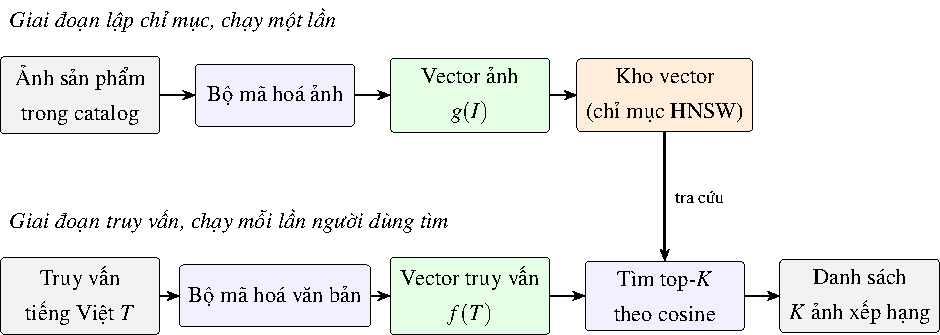
\includegraphics[width=0.96\textwidth]{graphics/fig_ch2_1.pdf}
\caption{Hai giai đoạn tìm kiếm dựa trên biểu diễn chung ảnh và văn bản}
\label{fig:ch2-pipeline}
\end{figure}

Hai không gian chỉ khớp nhau khi hai bộ mã hoá được huấn luyện chung, nên một bộ mã hoá văn bản tiếng Việt đơn mô thức không ghép trực tiếp được với bộ mã hoá ảnh của SigLIP~2. CLIP, SigLIP~2 và ViSigLIP-OT đều có sẵn cả bộ mã hoá ảnh lẫn bộ mã hoá văn bản: CLIP cho vector 512 chiều, SigLIP~2 và ViSigLIP-OT cho vector 768 chiều.
\subsection{Hàm mất mát tương phản}
\label{sec:ham-mat-mat}

Xét một lô gồm $B$ cặp ảnh--văn bản, với $x_i=g(I_i)$ và $y_i=f(T_i)$ là các vector đã chuẩn hoá. Logit của cặp $(i,j)$ là $z_{ij}=t\,x_i^{\top}y_j$, trong đó $t$ là hệ số tỷ lệ (nghịch đảo của nhiệt độ) được học cùng mô hình. CLIP coi cặp đúng $(i,i)$ là lớp đúng của một bài toán phân loại $B$ lớp và lấy entropy chéo theo cả hai chiều, từ ảnh sang văn bản và từ văn bản sang ảnh:
\begin{equation}
\mathcal{L}_{\mathrm{softmax}}=-\frac{1}{2B}\sum_{i=1}^{B}\left[\log\frac{e^{z_{ii}}}{\sum_{j=1}^{B}e^{z_{ij}}}+\log\frac{e^{z_{ii}}}{\sum_{j=1}^{B}e^{z_{ji}}}\right].
\label{eq:softmax}
\end{equation}
Mẫu số của mỗi số hạng cộng trên cả hàng hoặc cả cột, nên mọi phần tử khác trong lô đều là mẫu âm và chất lượng huấn luyện phụ thuộc cỡ lô $B$.

SigLIP bỏ phép chuẩn hoá này. Mỗi cặp $(i,j)$ là một bài toán phân loại nhị phân độc lập, với nhãn $\ell_{ij}=+1$ khi $i=j$ và $\ell_{ij}=-1$ trong các trường hợp còn lại; logit có thêm độ lệch $\beta$ học được, $z_{ij}=t\,x_i^{\top}y_j+\beta$. Bài báo gốc chia tổng cho $B$, còn đồ án chia cho $B^2$ (trung bình trên toàn bộ các cặp), nên giá trị mất mát nhỏ hơn $B$ lần:
\begin{equation}
\mathcal{L}_{\mathrm{sigmoid}}=-\frac{1}{B^{2}}\sum_{i=1}^{B}\sum_{j=1}^{B}\log\sigma\!\left(\ell_{ij}\,z_{ij}\right),\qquad \sigma(u)=\frac{1}{1+e^{-u}}.
\label{eq:sigmoid}
\end{equation}
Hình~\ref{fig:ch2-loss} đặt hai cách tính cạnh nhau trên ma trận độ tương đồng của một lô bốn cặp: ở CLIP, mỗi phép softmax phải nhìn thấy cả hàng (hoặc cả cột) tương ứng, còn ở SigLIP mỗi ô được chấm độc lập. Đồ án huấn luyện bằng hàm mất mát sigmoid theo cặp.

Mẫu âm khó của một sản phẩm là các sản phẩm gần nó nhất nhưng không phải cặp đúng; chúng làm bài toán phân biệt khó hơn so với mẫu âm ngẫu nhiên trong lô. Cách chọn mẫu âm khó của đồ án trình bày ở Mục~\ref{sec:tinh-chinh}.

\begin{figure}[H]
\centering
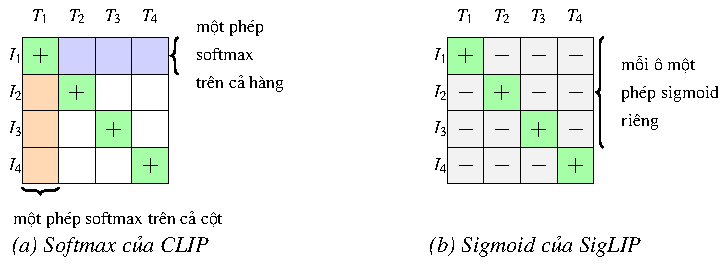
\includegraphics[width=0.9\textwidth]{graphics/fig_ch2_2.pdf}
\caption{So sánh hàm mất mát softmax và sigmoid trên ma trận độ tương đồng của một lô bốn cặp}
\label{fig:ch2-loss}
\end{figure}

\subsection{Tìm kiếm thưa BM25}
\label{sec:bm25}

BM25 chấm điểm một tài liệu $d$ cho truy vấn $q$ bằng cách cộng đóng góp của từng từ $w$ trong truy vấn:
\begin{equation}
\mathrm{BM25}(q,d)=\sum_{w\in q}\mathrm{IDF}(w)\cdot\frac{\mathrm{tf}(w,d)\,(k_1+1)}{\mathrm{tf}(w,d)+k_1\left(1-b+b\,\dfrac{|d|}{\mathrm{avgdl}}\right)},
\label{eq:bm25}
\end{equation}
trong đó $\mathrm{IDF}(w)=\ln\dfrac{N-n_w+0{,}5}{n_w+0{,}5}$, $\mathrm{tf}(w,d)$ là số lần từ $w$ xuất hiện trong $d$, $|d|$ là độ dài $d$, $\mathrm{avgdl}$ là độ dài trung bình của tài liệu, $N$ là số tài liệu và $n_w$ là số tài liệu chứa $w$. Tham số $k_1$ giới hạn mức tăng điểm theo tần suất từ, còn $b$ điều chỉnh mức phạt tài liệu dài. IDF của một từ có mặt trong hơn nửa số tài liệu sẽ âm; cài đặt của đồ án thay giá trị âm bằng một giá trị dương nhỏ, là $0{,}25$ lần IDF trung bình.

\subsection{Tìm kiếm vector gần đúng}
\label{sec:tim-kiem-gan-dung}

Với vector đã chuẩn hoá, xếp hạng theo cosine tương đương xếp hạng theo khoảng cách $L_2$. HNSW giảm chi phí này bằng đồ thị nhiều tầng: tầng trên cùng thưa, mỗi tầng dưới thêm nhiều nút hơn, và truy vấn đi tham lam từ tầng trên xuống để tới vùng chứa láng giềng gần nhất. Các tham số của đồ thị quyết định đánh đổi giữa tốc độ và tỷ lệ tìm đúng láng giềng thật.

\subsection{Tinh chỉnh hiệu quả tham số}
\label{sec:tinh-chinh-ly-thuyet}

Với ma trận trọng số gốc $W_0\in\mathbb{R}^{d_{\mathrm{out}}\times d_{\mathrm{in}}}$ được giữ cố định, LoRA học hai ma trận $U\in\mathbb{R}^{d_{\mathrm{out}}\times r}$ và $V\in\mathbb{R}^{r\times d_{\mathrm{in}}}$ với hạng $r\ll\min(d_{\mathrm{out}},d_{\mathrm{in}})$ và cộng tích của chúng vào trọng số gốc:
\begin{equation}
W=W_0+\frac{\alpha}{r}\,UV.
\label{eq:lora}
\end{equation}
DoRA tách trọng số thành độ lớn $m$ (vector học được) và hướng, rồi chỉ dùng phần cập nhật hạng thấp để điều chỉnh hướng. Với $W'=W_0+\frac{\alpha}{r}UV$, vector $m\in\mathbb{R}^{d_{\mathrm{out}}}$ có một phần tử cho mỗi đầu ra, và $\lVert W'\rVert_{\mathrm{row}}\in\mathbb{R}^{d_{\mathrm{out}}}$ là chuẩn $L_2$ của từng hàng $W'$ (mỗi hàng ứng với một đầu ra):
\begin{equation}
W=\mathrm{diag}(m)\,\mathrm{diag}\bigl(\lVert W'\rVert_{\mathrm{row}}\bigr)^{-1}W'.
\label{eq:dora}
\end{equation}

\subsection{Chỉ số đánh giá}
\label{sec:chi-so-danh-gia}

Mỗi cặp truy vấn--sản phẩm do người chấm xem được ít nhất hai người chấm độc lập theo thang 0 (không liên quan), 1 (liên quan một phần) và 2 (liên quan chính xác). Điểm của cặp là trung bình các điểm đó, nên có thể nhận giá trị lẻ như 0,5 hoặc 1,5; cặp được tính là liên quan khi điểm trung bình từ 1 trở lên. Cặp xuất hiện trong $K$ kết quả đầu mà chưa có nhãn được tính là không liên quan. Độ đồng thuận giữa các người chấm đo bằng hệ số kappa của Cohen~\cite{cohen1960kappa} và diễn giải theo thang của Landis và Koch~\cite{landis1977kappa}.

Gọi $Q$ là tập truy vấn, $D^{q}_i$ là kết quả hạng $i$ của truy vấn $q$ và $\mathbb{1}_{\mathrm{rel}}(q,D)$ cho biết cặp liên quan hay không. Recall@$K$ trong đồ án là tỷ lệ truy vấn có ít nhất một kết quả liên quan trong $K$ kết quả đầu. Đây là tỷ lệ trúng, khác với cách BEIR~\cite{thakur2021beir} tính Recall theo tỷ lệ tài liệu liên quan tìm lại được, nên số liệu hai bên không đặt cạnh nhau được:
\begin{equation}
\mathrm{Recall@}K=\frac{1}{|Q|}\sum_{q\in Q}\mathbb{1}\Bigl[\exists\, i\le K:\ \mathbb{1}_{\mathrm{rel}}\bigl(q,D^{q}_i\bigr)\Bigr].
\label{eq:recall}
\end{equation}
MRR lấy trung bình nghịch đảo hạng của kết quả liên quan đầu tiên, $r_q$; số hạng của truy vấn không có kết quả liên quan trong danh sách bằng 0:
\begin{equation}
\mathrm{MRR}=\frac{1}{|Q|}\sum_{q\in Q}\frac{1}{r_q}.
\label{eq:mrr}
\end{equation}
nDCG@$K$ dùng điểm liên quan $\mathrm{rel}_i$ của kết quả hạng $i$. Mỗi kết quả đóng góp $2^{\mathrm{rel}_i}-1$ điểm, giảm dần theo logarit của hạng; IDCG là DCG của thứ tự lý tưởng, tính trên các cặp đã có nhãn của cùng truy vấn:
\begin{equation}
\mathrm{nDCG@}K=\frac{\mathrm{DCG@}K}{\mathrm{IDCG@}K},\qquad \mathrm{DCG@}K=\sum_{i=1}^{K}\frac{2^{\mathrm{rel}_i}-1}{\log_2(i+1)}.
\label{eq:ndcg}
\end{equation}
Đồ án loại khỏi trung bình nDCG những truy vấn không có cặp nào đạt điểm liên quan từ 1 trở lên, vì IDCG của chúng bằng 0. Recall và MRR vẫn giữ các truy vấn này với giá trị 0, nên mẫu số của ba chỉ số không giống nhau.

Để so sánh hai hệ $S_1$ và $S_2$ trên cùng tập truy vấn, đồ án dùng kiểm định bootstrap ghép cặp theo truy vấn. Gọi $\Delta$ là hiệu trung bình của chỉ số theo từng truy vấn giữa $S_1$ và $S_2$. Phép kiểm định lấy mẫu lại các truy vấn có hoàn lại $R$ lần, tính $\Delta^{*}_r$ trên mỗi lần lấy mẫu, và khi $\Delta>0$ thì giá trị $p$ hai phía là
\begin{equation}
p=\frac{2}{R}\sum_{r=1}^{R}\mathbb{1}\bigl[\Delta^{*}_r\le 0\bigr],
\label{eq:bootstrap}
\end{equation}
với dấu bất đẳng thức đổi chiều khi $\Delta<0$, và $p$ được giới hạn ở 1. Đồ án không hiệu chỉnh các giá trị $p$ cho nhiều phép so sánh.
